\subsection{Satteins}
Das Testgebiet des Systems war in Satteins. In den folgenden Punkten wird kurz das Gebiet beschrieben und wie die Daten erfasst wurden.
\subsubsection{Topologie}
Im nachfolgenen Bild (\fref{bSatteins}) ist die Topologie von Satteins dargestellt. In dieser Darstellung sind die Aufstellpunkte der sechs aufgestellten Geräte mit einem schwarzen Punkt schematisch markiert. Jedes dieser Geräte wurde an den Ein- und Ausfahrtspunkten, sowie an strategisch interessanten Verkehrspunkten platziert. Mit diesen sechs Geräten ist es möglich, den grössten Teil des Verkehrsflusses in Satteins quantitativ zu rekonstruieren. 

\begin{figure}[H]
  \centering
  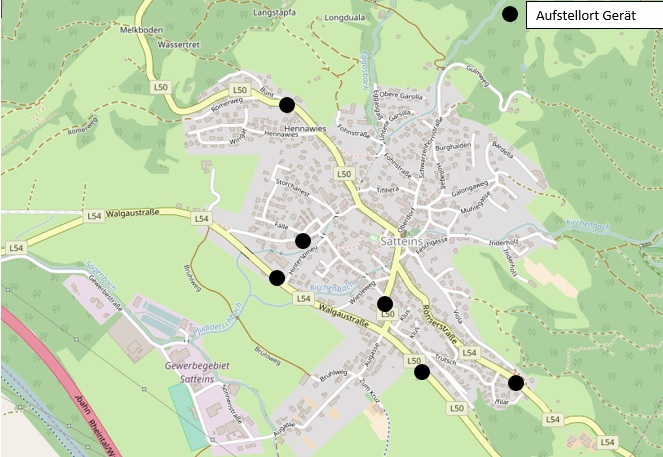
\includegraphics[width=0.99\textwidth]{Resultate/Satteins.jpg} 
  \caption{Topologie von Satteins. \cite{satteins}}
  \label{bSatteins}
\end{figure}

Mit Hilfe des Bildes (\fref{bGraph}) wird jede Abzweigung welche die Verkehrsteilnehmer nehmen können identifiziert und in der Berechnung des Verkehrsflusses beachtet. Dabei werden die Geräte schematisch auf einen Knotenpunkt, bei den Ein- und Ausfahrtsstrassen gelegt und die zwei Anderen werden auf die Mitte der Strasse projiziert. So lässt sich der Verkehrsfluss im Graphen darstellen und zu Letzt auf die Karte von Satteins zurück projizieren.

\begin{figure}[H]
  \centering
  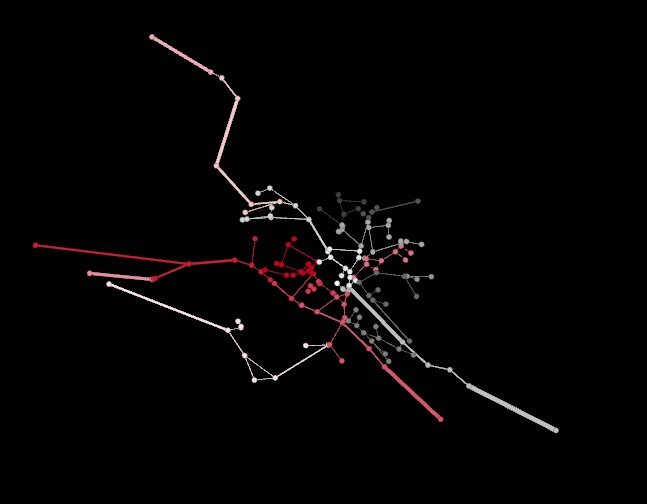
\includegraphics[width=0.99\textwidth]{Resultate/Topologie.jpg} 
  \caption{Graph des Verkehrsnetzes von Satteins.}
  \label{bGraph}
\end{figure}

\subsubsection{Erfassung der Daten}
Alle Daten welche die Geräte aufgezeichnet haben, wurden auf den internen SD-Karten abgespeichert und jeden zweiten Tag mittels Smartphone-Hotspot auf den Laptop übertragen. Dabei wurde bei jedem einzelnen Gerät der Feature Vektor, sowie der Temperaturverlauf heruntergeladen. Die Feature Vektoren der Geräte enthielten mehrere tausend Einträge mit vorbeifahrenden Verkehrsteilnehmern.